\RequirePackage{plautopatch}
\RequirePackage[l2tabu, orthodox]{nag}

\documentclass[uplatex,dvipdfmx]{jsarticle}
\usepackage{osukalab_pub_doc}
\usepackage{epic,eepic}
\usepackage{graphicx}
\usepackage{amsmath}
\usepackage[all, warning]{onlyamsmath}
\usepackage{siunitx}
\usepackage{txfonts}
\usepackage{amssymb}

\pagestyle{empty}

%%%%% 図を貼るまでの仮置き枠．図を用意したら \includegraphics に置き換える
%%%%% 使い方：\figplaceholder{幅}{メモ}
\newcommand{\figplaceholder}[2]{%
  \fbox{\parbox[c][0.45#1][c]{0.95#1}{\centering\small TODO：#2}}}

%%%%% 本文を書いたら消す目印（PDF上で赤字にしたいなら xcolor を入れて色付けしてもよい）
\newcommand{\todo}[1]{\textbf{【TODO：#1】}}

\headding{浪花研研究会}

\title{地形周波数表現による移動ロボットの走行性能の評価\\ {\Large ---一定トルク駆動における定常走行条件の構築と車輪径の影響---} }
% ↑副題は仮．SI2026と同じ「車輪径と走行性能の関係性の検証」のままでもよい

\department{機械工学専攻}
\laboratory{フィールドロコモーション研究室}
\author{佐藤 翔亮}

\date{2026年11月19日}

\begin{document}

\maketitle
\thispagestyle{empty}

%====================================================================
\section{緒言}
%====================================================================
% 前回（document.tex）の緒言をそのまま流用．研究会の聴き手は背景を知っているので，
% 長ければ2段落程度に削ってよい．

災害大国である日本では，不整地環境で活動可能な小型移動ロボットの需要が高い．
このような移動ロボットは，複雑な環境での走破性を向上させるために，設計段階から多様なアプローチが考えられてきた．
代表的な例として，複数の移動機構の併用および合体
\cite{Quince,TITANXX,trackwalker,iRobotPackBot}，
新たな移動機構の開発
\cite{DFC,Mecanum_wheel}，
生物に着想を得た移動機構の検証
\cite{asterisk,harvestman_robot,i_centipod_aqua,K3,six_legged_robot}
等が挙げられる．
先行研究における不整地走破性能の評価方法は，段差の高さや斜度，間隙の長さなどのスケールを用いた指標や
\cite{TITANXX,DFC,six_legged_robot,ro-ba}，
ロボットフィールドや実際の災害現場のような特定の環境内における速度や走破可否といった性能によって検証されてきた
\cite{Quince,trackwalker,i_centipod_aqua}．
しかしながら，このような評価方法では個別の状況・条件における性能しか比較できず，実際の現場が同様の環境であるとは限らない．

そこで本研究では，不整地の路面形状を空間的な波形として捉え，その不整地における走行性能を波形の振幅と空間周波数に対する応答として評価する手法の構築を目指す(Fig.~\ref{fig:概要図})．

\begin{figure}[tb!]
    \centering
    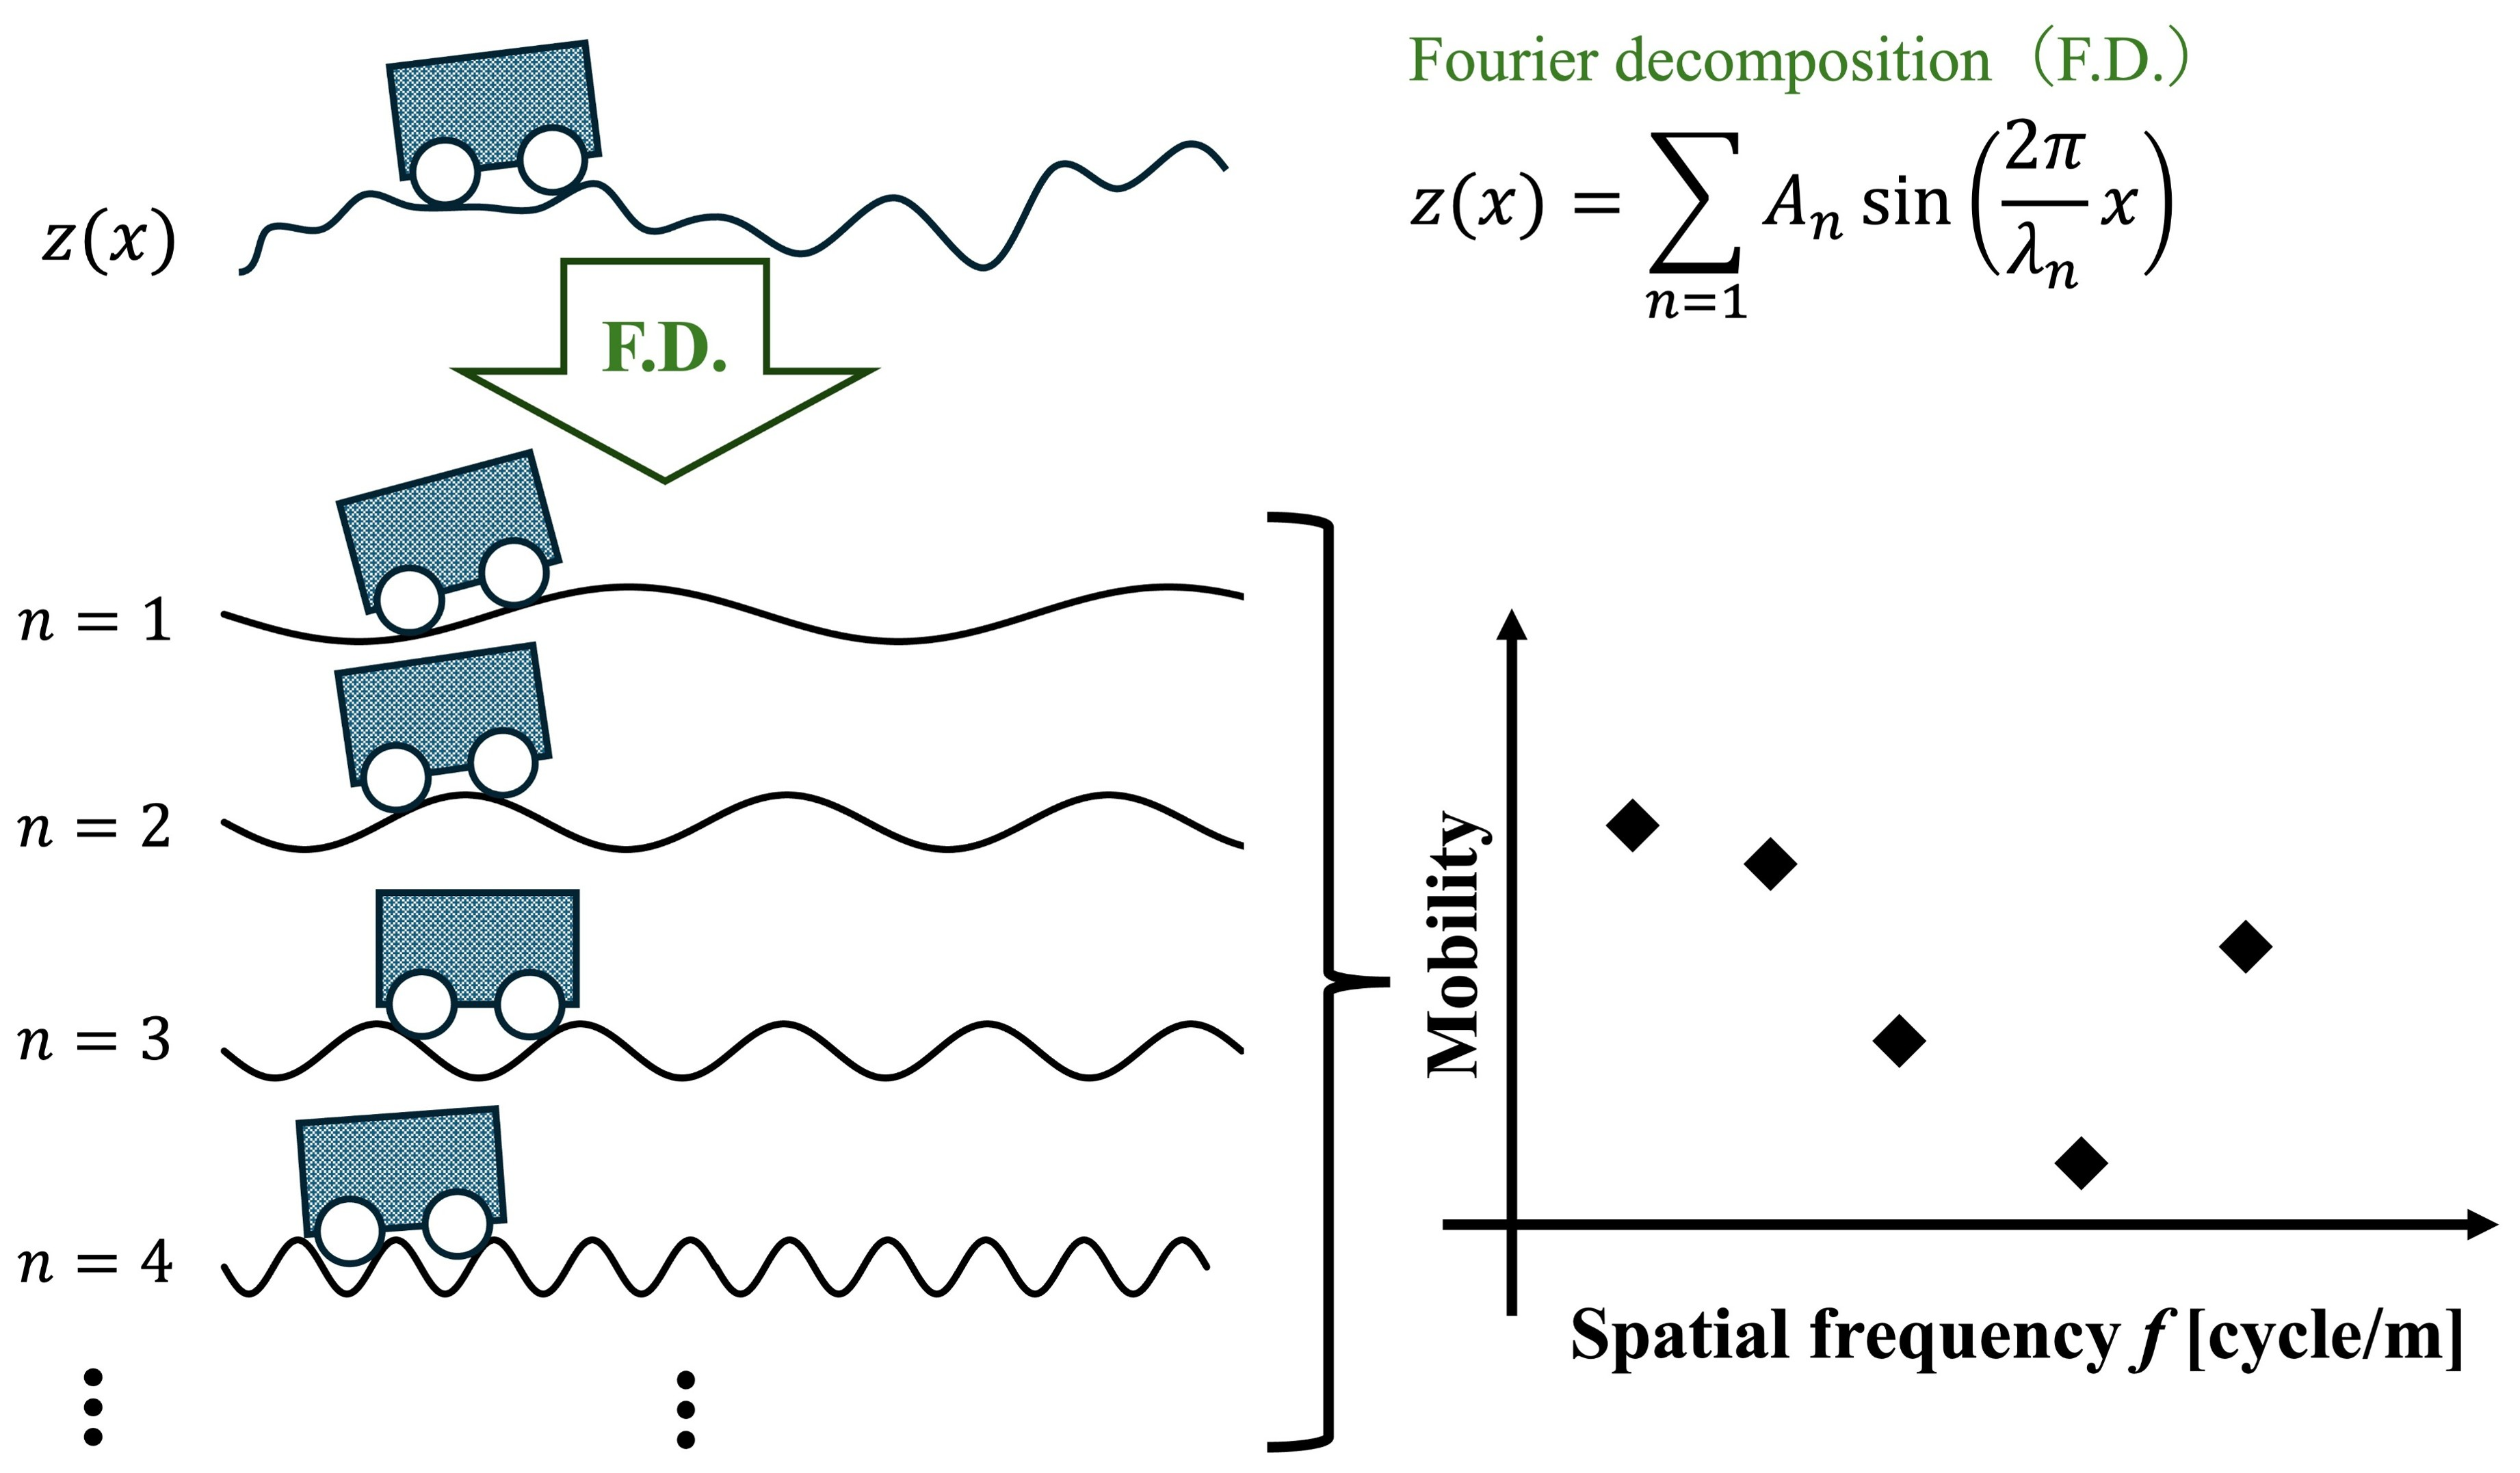
\includegraphics[width=1.0\linewidth]{figure/concept2.jpg}
    \caption{Concept of mobility evaluation using terrain frequency representation}
    \label{fig:概要図}
\end{figure}

% ---- ここから今回追記する部分 ----
\todo{前報までの位置づけを書く}
% 書くこと：
%  ・RM2026\cite{myproceedings}：車両固定・振幅を変えて，周波数領域での評価が有効なことを確認
%  ・SI2026\cite{SI2026}：車輪径を7水準に変えた（τ=10 N·m，抵抗なし，静止から加速）
%  ・ただし両者とも「加速途中（過渡状態）のデータ」だったことが後で分かった
%  ・本稿：定常走行で比較できる条件を作り直し，車輪径の影響を再検証した → 何が分かって何が残ったか
%
% 問い返し：聴き手に「なぜ過渡状態だと困るのか」を1文で言えるか？
%   （ヒント：同じ地形でも，進入時の速度が車輪径ごとに違うと，何の差を見ていることになるか）

%====================================================================
\section{前報（SI2026）までの取り組みと問題点}
%====================================================================

\subsection{評価方法の概要}
% SI2026 2.1節の内容を短くまとめる．図はSI2026のsimimage/simscreenshotが流用できる．
\todo{評価方法の要約（空間周波数 $f = 1/\lambda$，矢状面拘束，評価量）}

\begin{figure*}[t!]
	\centering
	\begin{subfigure}{0.6\textwidth}
		\centering
		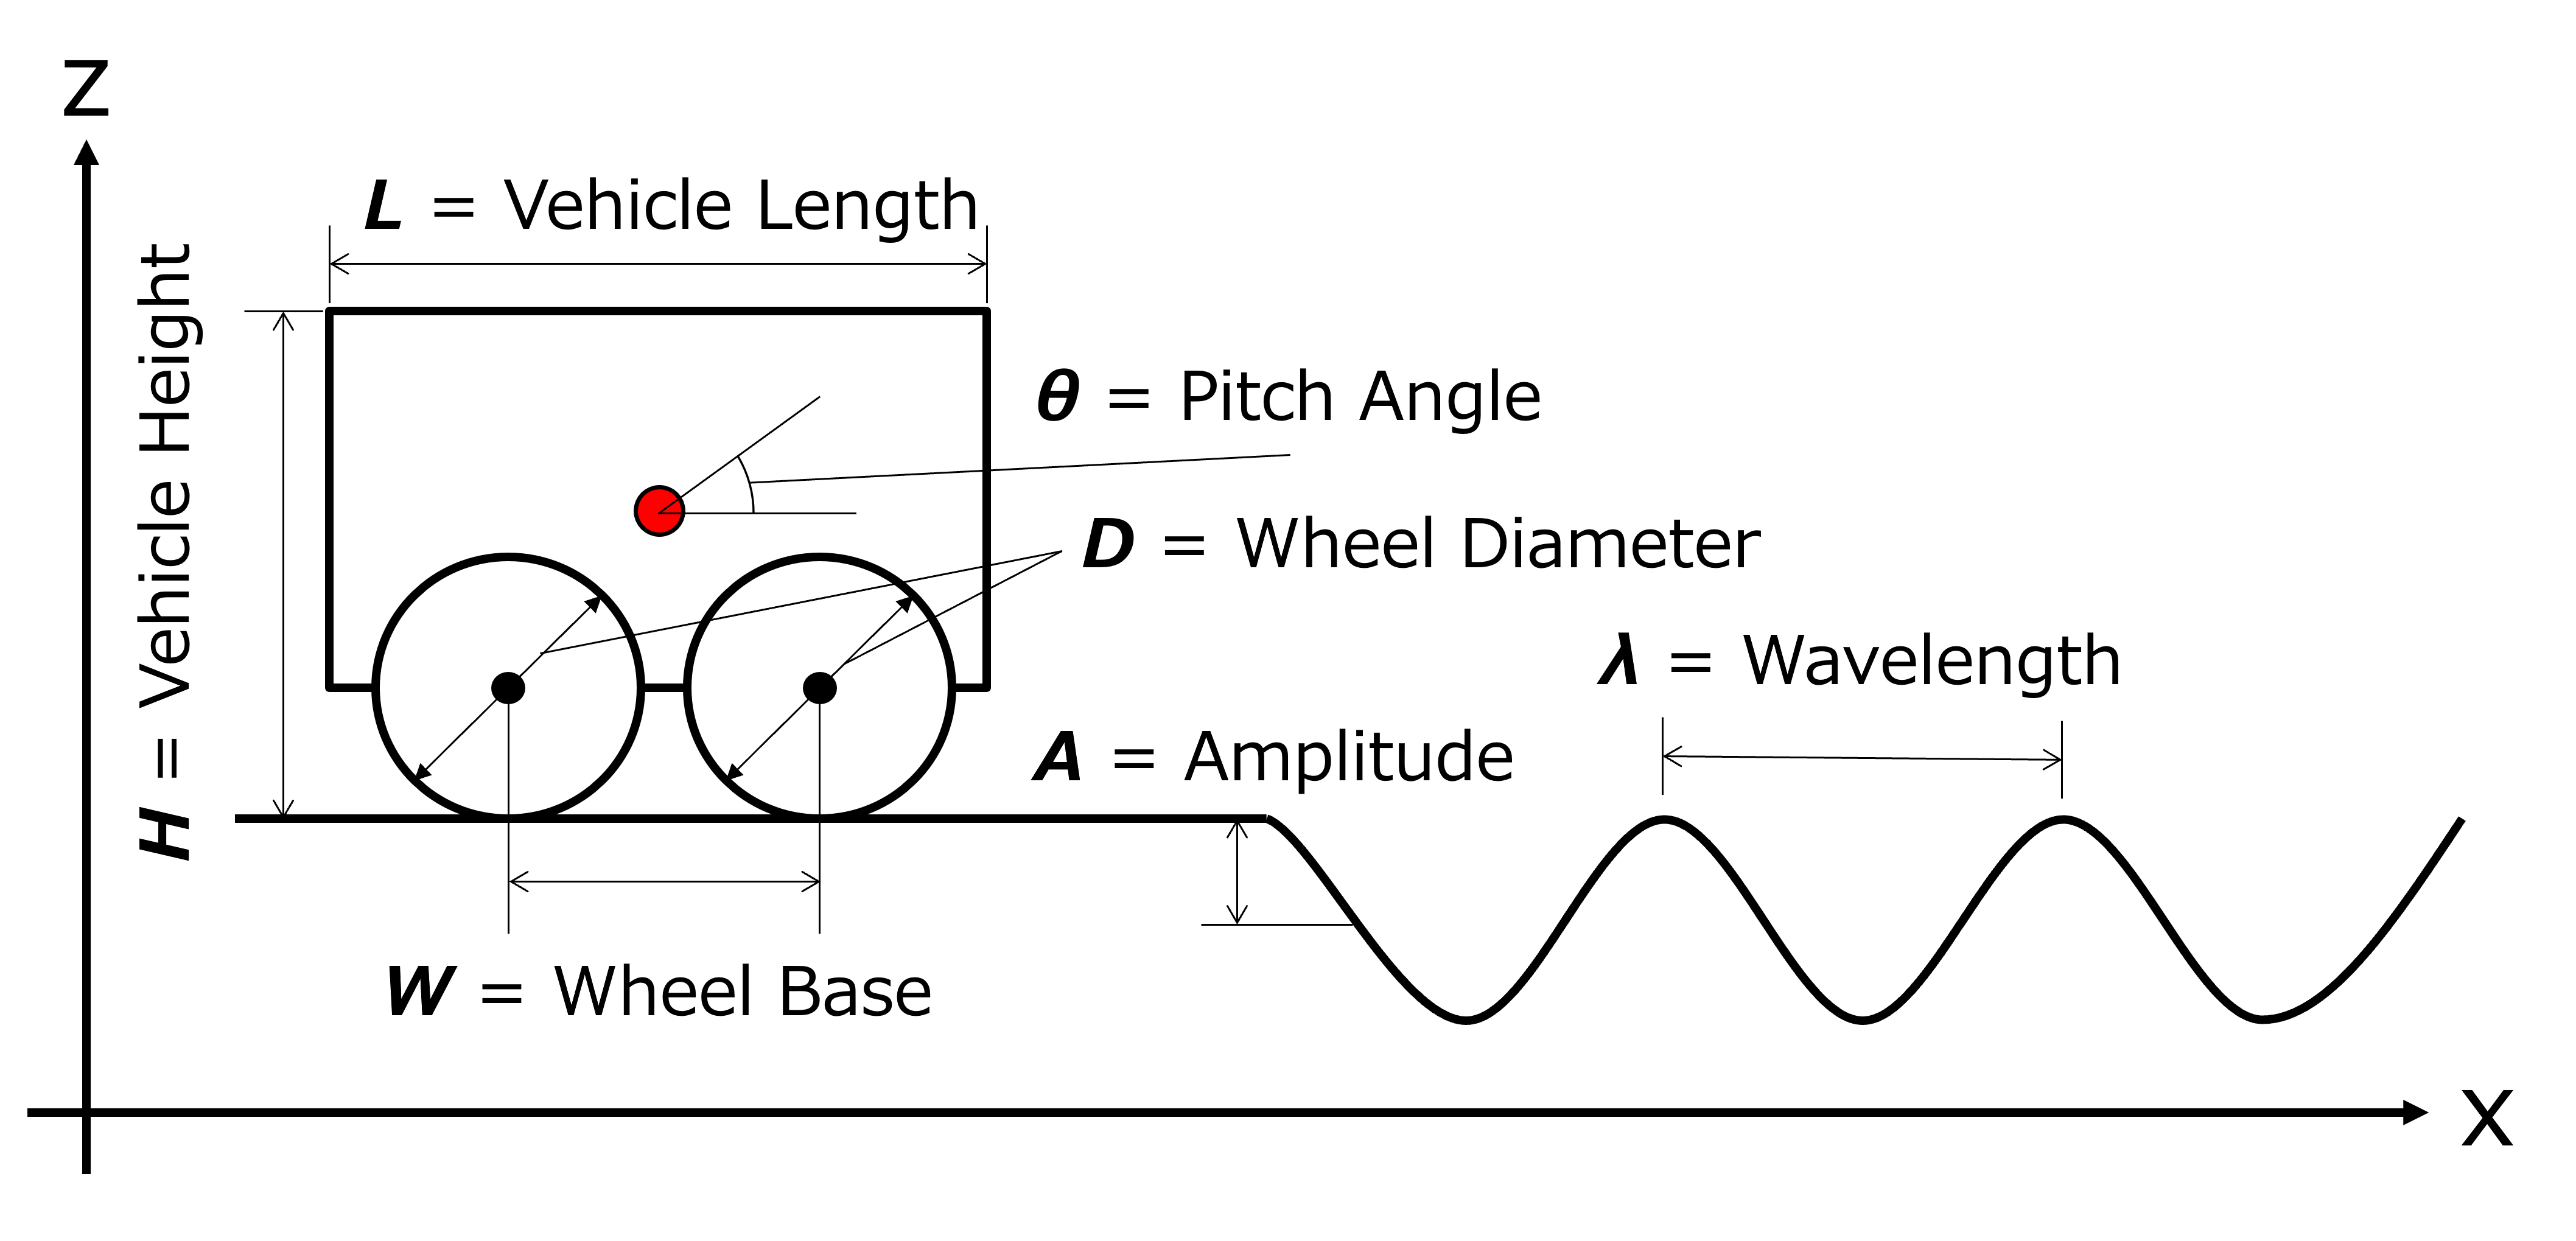
\includegraphics[width=\linewidth]{figure/simimage.png}
		\caption{Simulation of mobility evaluation using frequency characteristics}
		\label{fig:simのイメージ図}
	\end{subfigure}
	\hspace{0.05\textwidth}
	\begin{subfigure}{0.3\textwidth}
		\centering
		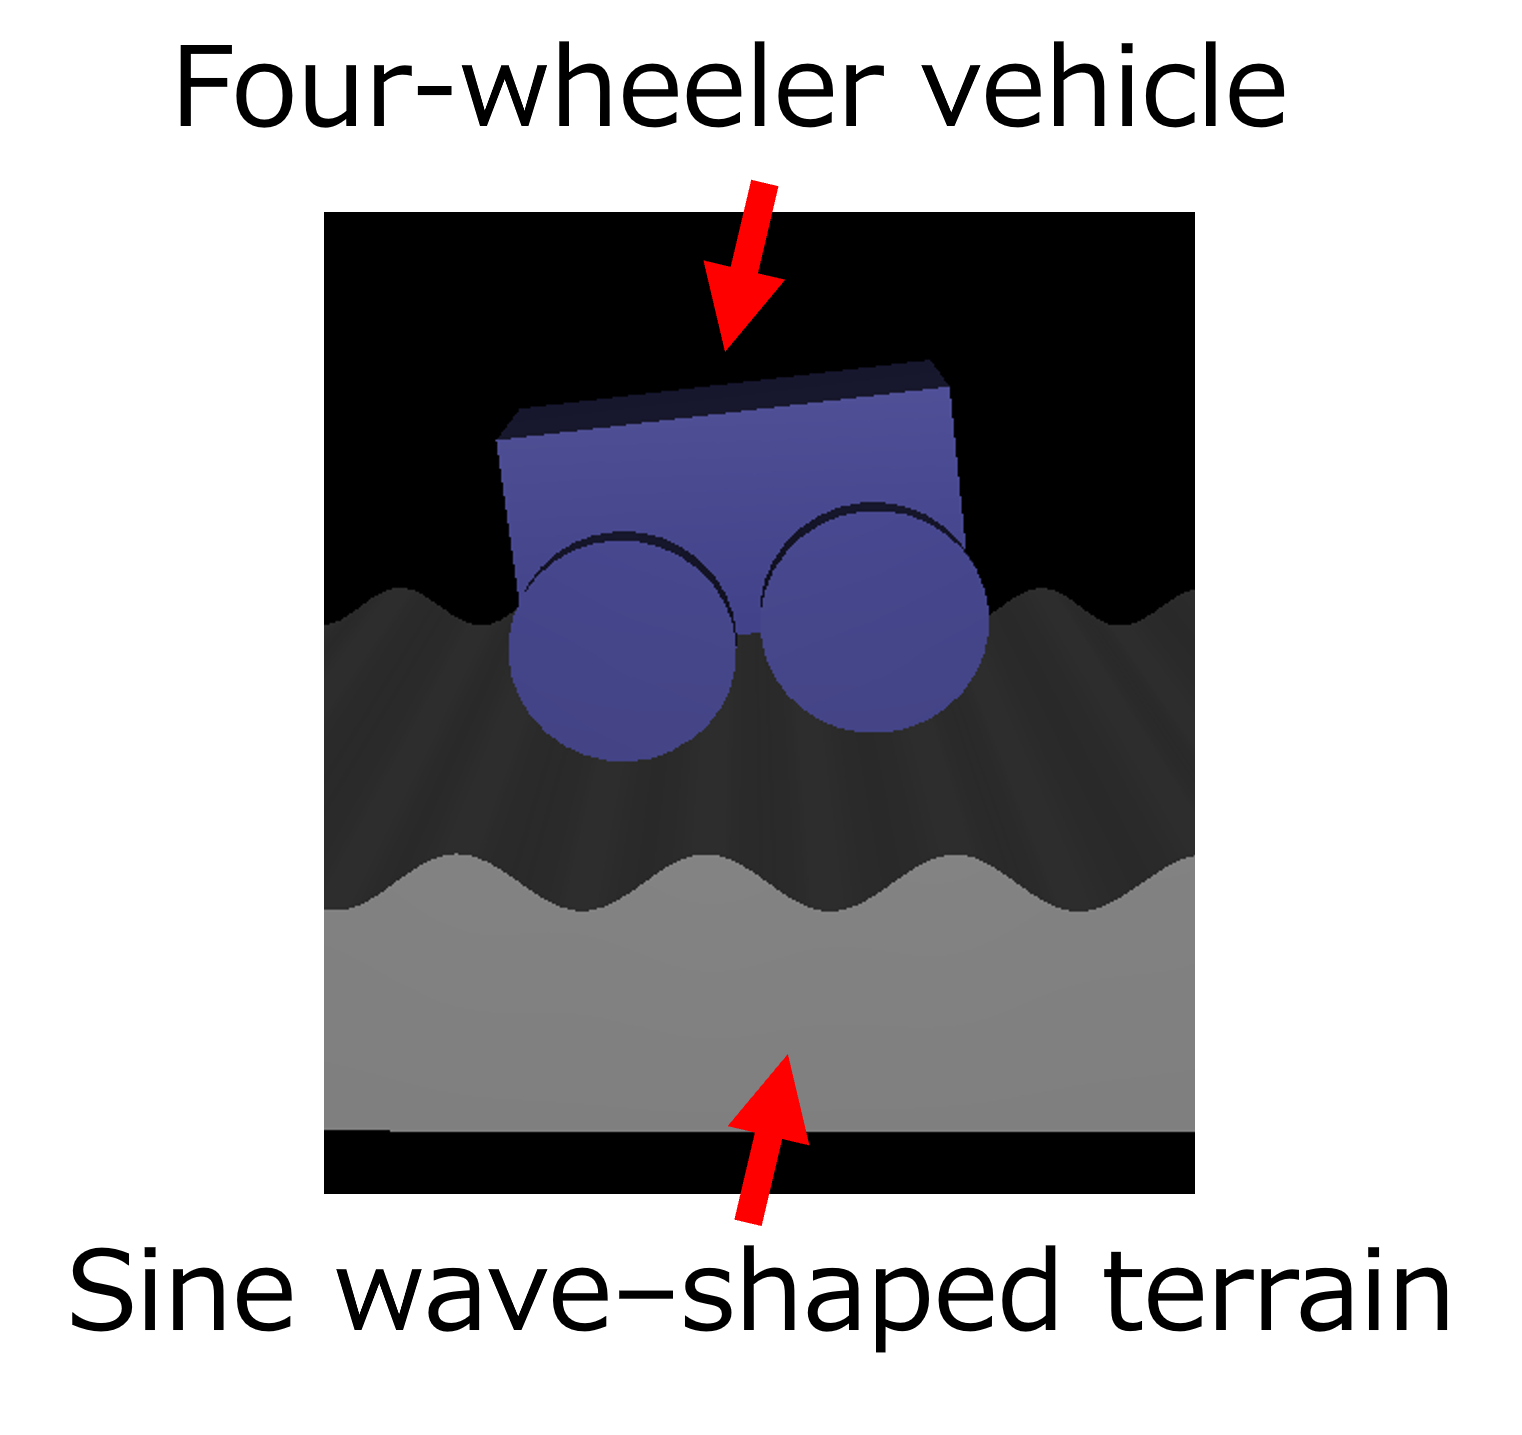
\includegraphics[width=\linewidth]{figure/simshot.png}
		\caption{Screenshot of simulation}
		\label{fig:simスクショ}
	\end{subfigure}
	\caption{Overall structure and screenshot of the simulation}
	\label{fig:まとめ図}
\end{figure*}

\subsection{SI2026の結果と，その後に判明した問題}
\todo{SI2026の主張を2〜3点に要約し，それぞれの問題点を書く}
% 書くこと（引き継ぎメモ5章・7章より）：
%  ・SI2026のデータは τ=10 N·m，抵抗なし → 平地でも速度が増え続け，定常にならない
%    （抵抗なしで20秒走ると13.9 m/s に達し，頭打ちにならない）
%  ・つまり「平均速度」は地形の影響と加速の過渡が混ざった量だった
%  ・SI2026で計測量に挙げた鉛直速度 V_z は9月以前のデータでは無効（4章の不具合1）
%  ・SI2026の「大径ほど走行速度は遅い（当然）」は，抵抗の入れ方次第で逆転する（6章）
%
% 問い返し：SI2026の表では車体高さ0.75 m，メモでは0.5 m になっている．どちらが正しいか
%   config.yaml で確認しておくこと（質疑で聞かれたときに即答できるように）．

%====================================================================
\section{一定トルク駆動における定常走行条件の構築}
%====================================================================

\subsection{一定トルクでは定常状態にならない問題}
% 下の式は引き継ぎメモ2章より．式の導出（なぜ +5 kg になるか）は自分で説明できるようにしておくこと．
車輪を円板とみなすと，並進方向の等価質量 $m_{\mathrm{eff}}$ と推進力 $F$ は
\begin{align}
  m_{\mathrm{eff}} &= m + \frac{4I}{r^{2}} = m + 2m_{\mathrm{w}} = \SI{65}{kg}
  \label{eq:meff}\\
  F &= \frac{4\tau}{r}
  \label{eq:force}
\end{align}
となる．ここで $m = \SI{60}{kg}$ は総質量，$m_{\mathrm{w}} = \SI{2.5}{kg}$ は車輪1輪の質量，$I$ は車輪の慣性モーメント，$r$ は車輪半径，$\tau$ は1輪あたりの駆動トルクである．
\todo{抵抗がないと平地で $\dot v = F/m_{\mathrm{eff}}$ のまま加速し続けることを説明する}

\subsection{走行抵抗の導入方法}
\todo{3方式の説明．「どれも実在の抵抗を測った値ではなく，定常状態を作るための仮想的な粘性である」ことを必ず明記}

\begin{table}[t!]
    \caption{Three methods of introducing running resistance}
    \label{tab:drag_methods}
    \centering
    \scalebox{0.72}{
    \begin{tabular}{lccc}\hline
     Method & Resistance & Steady speed $v_{\mathrm{ss}}$ & Time constant $T$ \\ \hline\hline
     Body drag   & $-c\,v$ (force)        & $4\tau/(c\,r)$          & $m_{\mathrm{eff}}/c$ \\
     Axle damping & $-b\,\omega$ (torque) & $\tau\,r/b$             & $m_{\mathrm{eff}}\,r^{2}/(4b)$ \\
     Fluid drag  & $\propto v^{2}$         & $\sqrt{4\tau/(r\,k)}$   & --- \\ \hline
    \end{tabular}
    }
\end{table}

% 車体抵抗：car1_slide_x の damping，車軸の粘性：4輪ヒンジの damping，媒質抵抗：<option density viscosity>
% 4b/r^2 = c と置くと車体抵抗と同じ形になる → 同じ b でも小径では強く，大径では弱く効く
%
% 問い返し：Table~\ref{tab:drag_methods} の v_ss の式から，車輪径を大きくしたとき
%   車体抵抗方式と車軸方式で定常速度がそれぞれ上がるか下がるかを，式だけで言えるか？
%   これが7章の「結論が反転する」問題の核心になる．

\subsubsection{検討して却下した案：地形側だけで定常状態を作る}
\todo{凹凸の損失・転がり摩擦・接触の柔らかさの3案と，それぞれ不可とした理由}
% メモ2章：λ=400 px／A=0.05 m は90 m走っても加速し続けた，など実測の根拠を添える

\subsection{定常速度の較正と収束判定}
\todo{平地で定常速度を実測し，その速度を初速として地形に進入させる仕組みの説明}

\begin{table}[t!]
    \caption{Convergence criteria for steady speed}
    \label{tab:steady_criteria}
    \centering
    \scalebox{0.8}{
    \begin{tabular}{ll}\hline
     Item & Value \\ \hline\hline
     Exclusion of start-up & first $\max(3T,\ \SI{2}{s})$ \\
     Evaluation block & \SI{2}{s} \\
     Criterion & std / mean in block $< \SI{1}{\percent}$ \\
     Minimum duration & \SI{10}{s} \\
     Maximum duration & \SI{60}{s} (else \texttt{converged: false}) \\ \hline
    \end{tabular}
    }
\end{table}

\todo{しきい値1\%と最短10秒の根拠を書く}
% メモ3章：
%  ・1%：7水準の平地30秒のばらつきが，健全 0.34〜0.53% と問題あり 2.1〜21% の2群に分かれた → 中間
%  ・10秒：D=125 mm, c=120 で自励振動が8〜12秒かけて成長．3秒で打ち切ると真値より27%高い値を拾う
%  ・ドリフトは記録のみ（判定に入れても合否は一致，速度差は最大0.5%）
%  ・文献では分野共通の「何%」はなく，ケース依存とされていた
%    → 文献を引用するなら，書誌情報は原典で必ず確認すること（AIが出した文献情報は捏造の可能性あり）

%====================================================================
\section{データの信頼性に関わる不具合の修正}
%====================================================================
% 研究会では「何が壊れていて，どのデータが使えなくなったか」が伝われば十分．
% 表は自分で埋める．行の候補（メモ4章）：
%  鉛直速度の記録ミス／バッチ途中のトルク混入／描画とバッチのモデル食い違い／転がり摩擦が無効（condim=3）／
%  レポートからの起動条件の欠落
\todo{不具合・影響・対処の表（Table~\ref{tab:bugs}）を埋める}

\begin{table}[t!]
    \caption{Bugs found and their impact on data}
    \label{tab:bugs}
    \centering
    \scalebox{0.8}{
    \begin{tabular}{p{0.3\linewidth}p{0.3\linewidth}p{0.3\linewidth}}\hline
     Bug & Impact & Fix \\ \hline\hline
      &  &  \\
      &  &  \\
      &  &  \\ \hline
    \end{tabular}
    }
\end{table}

%====================================================================
\section{シミュレーション条件}
%====================================================================
% 値は引き継ぎメモ8章より．車体高さはSI2026（0.75 m）と食い違うので config.yaml で要確認．

\begin{table}[t!]
    \caption{Simulation conditions}
    \label{tab:conditions}
    \centering
    \scalebox{0.75}{
    \begin{tabular}{lcc}\hline
     Item & Symbol & Value \\ \hline\hline
     Vehicle length / width / height & $L, W, H$ & 1.0 / 0.5 / 0.5~m \todo{要確認} \\
     Body mass & $M$ & 50~kg \\
     Wheel mass (each) & $m_{\mathrm{w}}$ & 2.5~kg \\
     Total mass & $m$ & 60~kg \\
     Wheel diameter & $D$ & 0.125--0.875~m (7 levels) \\
     Wheelbase & $B$ & 0.50~m \\
     Driving torque (each wheel) & $\tau$ & 5~N$\cdot$m \\
     Body drag coefficient & $c$ & 20~N$\cdot$s/m \\
     Terrain amplitude & $A$ & 0.05, 0.1, 0.2~m \\
     Spatial frequency & $f$ & 0.1--50~cycle/m (111 points) \\
     Acceleration lane & & 2.5~m \\
     Terrain length & & 100~m \\
     Termination & & 50~m reached or 60~s \\
     Time step & $\Delta t$ & 0.002~s \\ \hline
    \end{tabular}
    }
\end{table}

\todo{評価量の定義（距離で切る統計窓）を書く}
% メモ9章：
%  ・velocity は qvel[0]＝車体の前後方向の並進速度（車輪の周速ではない）
%  ・窓：d0 = 助走路2.5 m + 過渡（波長の2倍，最低1 m），d1 = 到達距離を波長の整数倍に切り下げた点
%  ・注意：時間平均なので，窓内で停止した条件は停止中のサンプルが支配する
%    （例：λ=60 px / D=0.25 m / A=0.1 m で 時間平均0.019，距離重み平均1.81，移動中のみ0.80 m/s）
% 問い返し：「時間平均」と「距離重み平均」のどちらを評価量にすべきか？ 自分の考えを1つ持っておく．

%====================================================================
\section{結果}
%====================================================================

\subsection{標準条件（車体抵抗方式）における車輪径の影響}
% データ：wheel_202611021734（τ=5 N·m, c=20 N·s/m, 定常開始）

\begin{figure}[t!]
    \centering
    \figplaceholder{\linewidth}{平地比の速度 vs 空間周波数（fig\_a\_speed\_ratio\_vs\_frequency）}
    % \includegraphics[width=1.0\linewidth]{figure/fig_a_speed_ratio_vs_frequency.png}
    \caption{Speed ratio to flat ground versus spatial frequency $f$}
    \label{fig:speed_ratio}
\end{figure}

\begin{figure}[t!]
    \centering
    \figplaceholder{\linewidth}{走破が回復する波長 vs 車輪直径（fig\_c\_recovery\_wavelength）}
    % \includegraphics[width=1.0\linewidth]{figure/fig_c_recovery_wavelength.png}
    \caption{Recovery wavelength versus wheel diameter}
    \label{fig:recovery}
\end{figure}

\todo{Fig.~\ref{fig:speed_ratio}, \ref{fig:recovery} から読み取れることを書く}
% メモ5章の主張（確からしさの区別も書くこと）：
%  ・λ=0.20〜0.60 m（f=1.67〜5.0 cycle/m）は21条件すべてで50 m走破不可 ← ホイールベース0.5 m と同程度
%  ・走破できない帯域の高周波側の端は，車輪径を7倍にしても波長10〜20 cm の範囲でしか動かない
%  ・振幅を上げると帯域が低周波側に広がる
%  ・「大径ほど平地とみなせる範囲が広がる」は支持されない（回復周波数 D=125で10.0，D=875で6.25 cycle/m）
%  ・平地の定常速度の実測／理論比：D≥375 mm で 0.92〜0.95，D=125・250 mm は 0.58・0.75
% 問い返し：SI2026の考察（Fig.4：大径ほど谷に嵌らない）と，今回の「否定」は矛盾するか？
%   矛盾するなら，どちらのデータの何が違うから結論が変わったと言えるか？

\subsection{車軸の粘性方式における車輪径の影響}
% データ：wheel_202611111858（τ=10 N·m, b=0.25 N·m·s, 定常開始）
\todo{走破が回復する波長が車輪直径に比例（$\lambda \simeq 0.61D$）という結果を書く}

\begin{table}[t!]
    \caption{Steady speed on flat ground for the two methods}
    \label{tab:speed_compare}
    \centering
    \scalebox{0.85}{
    \begin{tabular}{lcc}\hline
     Method & $D = \SI{0.125}{m}$ & $D = \SI{0.875}{m}$ \\ \hline\hline
     Body drag ($c = 20$)     & \SI{9.3}{m/s} & \SI{2.1}{m/s} \\
     Axle damping ($b = 0.25$) & \SI{2.5}{m/s} & \SI{16.9}{m/s} \\ \hline
    \end{tabular}
    }
\end{table}

%====================================================================
\section{考察：車輪径の効果と走行速度の効果の分離}
%====================================================================
\todo{2方式で結論が変わる理由を，Table~\ref{tab:drag_methods} の式と Table~\ref{tab:speed_compare} を使って説明する}
% ここが今回の発表の山場．自分の言葉で書くこと．
% 問い返し：
%  ・「車輪径の効果」を調べたいとき，何を揃えて（固定して）比較すべきか？
%      速度？ トルク？ 推進力？ 車輪の角速度？ それぞれ揃えたときに何が変わってしまうか．
%  ・b ∝ r にすると全径で速度が揃うのはなぜか（v = τr/b に代入）．そのとき「抵抗の強さ」は径で揃っているか？

%====================================================================
\section{未解決の問題と相談したい事項}
%====================================================================
% 研究会で浪花先生・鈴木先生に判断をもらいたいことを，選択肢つきで書くと議論が早い．
% 候補（メモ6章）：
%  1. 車輪径と速度の分離：b∝r／トルクを径に比例／v^2 項を足す，のどれで行くか
%  2. 定常速度の二枝（車軸方式・D=875・τ=10 で 10.76 と 16.20 m/s）：静止から較正するか，両方記録するか，速度域を下げるか
%  3. 抵抗係数を全径共通にすると速度が7倍開く
%  4. トルクの効果を分離したデータがない
%  5. 転がり摩擦が無効（condim=3）．有効化するか
%  6. 鈴木先生提案の評価量（同じ高さを通過するたびの速度低下量，単位距離あたりのエネルギ損失）の実装
\todo{相談事項を優先度順に，それぞれ「選択肢」と「自分の案」をつけて書く}

%====================================================================
\section{まとめと今後の展望}
%====================================================================
\todo{まとめ}
% 短期：車輪径のシミュレーションを2027年3月までに一段落させる
% 中期：ホイールベース等の次のパラメータ，または実機

%====================================================================
\begin{thebibliography}{99}

\bibitem{Quince}
小柳 栄次, サブクローラを持つレスキューロボット, 日本ロボット学会誌, Vol.28, No.2 (2010), pp. 147--150

\bibitem{TITANXX}
程島竜一, 福村泰明, 天野久徳, 広瀬茂男, クローラ可変型4足歩行ロボットTITAN Xの開発, 日本ロボット学会誌, Vol.28, No.7 (2010), pp. 872--879

\bibitem{trackwalker}
永谷 圭司，秋山 健，吉田 和哉，西田 信一郎, J192011 揺動サイドクローラを有する移動ロボットTrackWalker II による不整地走行実験 : 三原山裹砂漠と中田島砂丘における走行試験, 年次大会, Vol.2012, (2012) pp. \_J192011--1--\_J192011--3

\bibitem{iRobotPackBot}
Jessica Gwozdz, N~Morin, Ransom~Philip Mowris, Enabling semi-autonomous manipulation on Irobot's Packbot, {\em Worcester Polytechnic Institute}, (2014)

\bibitem{DFC}
浪花 啓右，伊東 和輝，佐藤 悠弥，角田 祐輔，衣笠 哲也，谷口 寿俊，三谷 泰浩，大須賀 公一, 双胴柔軟クローラ型ロボット"d-FlexCraw"の走行時姿勢制御と直進性評価, ロボティクスメカトロニクス講演会講演概要集, Vol.2024, (2024) pp. 1A1--I05

\bibitem{Mecanum_wheel}
山田 紀之，古村 博隆，遠藤 玄，鈴森 康一, 螺旋形状を持つメカナムホイールによる全方向移動車両の不整地走行実験, ロボティクスメカトロニクス講演会講演概要集, Vol.2016, (2016) pp. 2A1--06b3

\bibitem{asterisk}
Tomohito Takubo, Tatsuo Arai, Kenji Inoue, Hikaru Ochi, Takeshi Konishi, Taisuke Tsurutani, Yasuo Hayashibara, Eiji Koyanagi, Integrated Limb Mechanism Robot ASTERISK, {\em Journal of Robotics and Mechatronics}, Vol.18, No.2 (2006), pp. 203--214

\bibitem{harvestman_robot}
程島 竜一, ザトウグモの形態を模倣した多脚ロボット, 日本ロボット学会誌, Vol.37, No.2 (2019), pp. 138--143

\bibitem{i_centipod_aqua}
山本 誠也，伊東 和輝，角田 祐輔，浪花 啓右，大須賀 公一, 水陸で立ち往生しない多脚ロボットの開発, システム制御情報学会　研究発表講演会講演論文集, Vol.SCI24, (2024) pp.~304--308

\bibitem{K3}
浪花 啓右，伊東 和輝，杉本 靖博，角田 祐輔，大須賀 公一, 徹底的に立ち往生しないことを目指した移動機構超多球面脚モジュールロボット：K3（KyuKyaKu）の平面構成走行, システム制御情報学会　研究発表講演会講演論文集, Vol.SCI23, (2023) pp.~1D1--06

\bibitem{six_legged_robot}
佐々木 大雅, 藤田 豊己, ６脚クローラ型不整地移動ロボットの開発と溝乗り越え運搬, ロボティクスメカトロニクス講演会講演概要集, Vol.2016, (2016) pp. 1P1--06b2

\bibitem{ro-ba}
長塩 拓馬，正岡 宏一，田中 耕治，二次元重心位置制御が可能な車輪型ローバの不整地での走行性能の検討, Proceedings of the 2016 JSME Conference on Robotics and Mechatronics, No.16-2, Yokohama, Japan, June 8-11, 2A2-18a3(1), 2016.

\bibitem{mujoco}
Emanuel Todorov, Tom Erez, Yuval Tassa, MuJoCo: A physics engine for model-based control, {\em 2012 IEEE/RSJ International Conference on Intelligent Robots and Systems}, pp.~5026--5033 (2012)

\bibitem{myproceedings}
佐藤 翔亮，鈴木 朱羅，大須賀 公一，浪花 啓右, 地形周波数表現による移動ロボットの走行性能の評価, ロボティクス・メカトロニクス講演会2026講演論文集, No.26-2, 2P2-O04 (2026)

\bibitem{SI2026}
佐藤 翔亮，鈴木 朱羅，大須賀 公一，浪花 啓右, 地形周波数表現による移動ロボットの走行性能の評価 ---車輪径と走行性能の関係性の検証---, \todo{SI2026の講演会名・講演番号・開催地・日付を記入}

\end{thebibliography}

\end{document}
